\phantomsection
\addcontentsline{toc}{subsection}{Imagination Technologies}
\subsect{Imagination Technologies - Dr David Knox - Senior Director Software Engineering}

Imagination technologies began in 1985, then known as Video Logic.
In 1999 the company moved toward IP licensing instead of manufacture and have since become a leading company in silicon, software and cloud technology~\cite{ImgHist}. Imagination has shipped 5 billion devices containing their IP, 1.2 billion of which were in 2013 \cite{ImgAnn13}.

Imagination is acquiring an increasingly diverse IP portfolio. In February 2013, it aquired the MIPS CPU architecture IP.
The company already had expertise in integrating Imagination and MIPS complementary technology.
MIPS provides the company an opportunity to enter the mobile processor market, as MIPS is one of the few CPU architectures supported by the Android OS \cite{ImgAnn13}. 
It remains to be seen if this related diversification will be successful for Imagination, especially when considering the success of the incumbant ARM.


Imagination also has a commercial electronics devision named Pure. 
The brand is synonymous with DAB radio, and allows Imagination a direct route to the consumer market.
Adopting the licensee business model adds the challenge of removal from the end user and customer.
By using Pure as a showcase for Imagination IP, an important line of feedback is developed.
The business model, shown in figure 1, is a multi-year cycle in which the Imagination use direct customer feedback to drive chip development for licensees.
This also gives Imagination an advisory role to OEMs regarding consumer preferences.
Imagination is a leading IP company with a diverse yet related portfolio of business opportunities which allow it be succesful.
 
\begin{figure}[!htb]
   \centering
   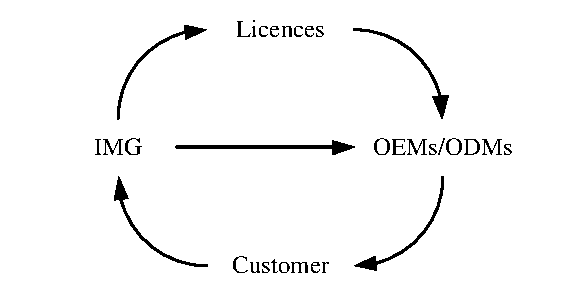
\includegraphics[width = 0.45\textwidth]{Figures/ImgModel.pdf}
   \label{figure:ImgModel}
   \caption{Imagination Technologies business model.}
\end{figure}
